% To be published in ApJ or Elsevier Astronomy and Computing
\documentclass{aastex62}
\usepackage[utf8]{inputenc}
\usepackage{natbib}
\usepackage{listings}
\usepackage{xspace}
\usepackage{paralist}
\usepackage{geometry}
\geometry{right=1.5in}

\newcommand{\package}[1]{\texttt{#1}\xspace}
\newcommand{\code}[1]{\texttt{#1}\xspace}

\newcommand{\github}{\package{GitHub}}

\newcommand{\python}{\package{Python}}

\newcommand{\sunpy}{SunPy\xspace}
\newcommand{\sunpyproj}{\sunpy project\xspace}
\newcommand{\sunpypkg}{\package{sunpy}}
\newcommand{\sunpycode}[1]{\code{#1}}

\newcommand{\astropy}{Astropy\xspace}
\newcommand{\astropypkg}{\package{astropy}}

\newcommand{\numpy}{NumPy\xspace}


\newcommand{\Map}{\sunpycode{Map}}
\newcommand{\Timeseries}{\sunpycode{TimeSeries}}
\newcommand{\Timeseriesmetadata}{\sunpycode{TimeSeriesMetaData}}
\newcommand{\Spectra}{\sunpycode{Spectra}}
\newcommand{\Fido}{\sunpycode{Fido}}
\newcommand{\Lightcurve}{\sunpycode{LightCurve}}
\newcommand{\GenericTimeSeries}{\sunpycode{GenericTimeSeries}}
\newcommand{\GenericMap}{\sunpycode{GenericMap}}

\newcommand{\hpc}{helioprojective Cartesian\xspace}
\newcommand{\hcc}{heliocentric Cartesian\xspace}
\newcommand{\hgs}{heliographic Stonyhurst\xspace}
\newcommand{\hgc}{heliographic Carrington\xspace}
\newcommand{\hpcframe}{\package{HelioprojectiveCartesian}}
\newcommand{\hccframe}{\package{HeliocentricCartesian}}
\newcommand{\hgsframe}{\package{HeliographicStonyhurst}}
\newcommand{\hgcframe}{\package{HeliographicCarrington}}

\shorttitle{Sunpy Project II}
\shortauthors{The Sunpy Community}

% Words that should not be hyphenated
\hyphenation{NumFOCUS}

% For commenting - can be deleted before submission
\usepackage[colorinlistoftodos]{todonotes}
\newcommand{\inlinecomment}[2]{\todo[inline]{#1: #2}\xspace}
\newcommand{\comment}[2]{\todo{#1: #2}\xspace}

\begin{document}

\title{The SunPy Project: Open Source Development and Status of the  v1.0 Core Package }
\author[0000-0000-0000-0000]{The SunPy Community}
\noaffiliation

% \author[orcid-id]{name}
% \affiliation{}

% below add contributing authors (those folks that have actually worked writing the paper) this list is alphabetical.
% daggers to recognize Stuart, Nabil, Jack, David.
% board members get some symbol next to their names.

\author[0000-0001-9642-6089]{Will T. Barnes}
\affiliation{Bay Area Environmental Research Institute, Petaluma, CA, USA}
\affiliation{Lockheed Martin Solar and Astrophysics Laboratory, Palo Alto, CA, USA}

\author[0000-0002-5662-9604]{Monica G.\ Bobra}
\affiliation{W.W. Hansen Experimental Physics Laboratory, Stanford University, Stanford, CA 94305, USA}
\affiliation{SunPy Board Member}

\author[0000-0001-6127-795X]{Steven D. Christe}
\affiliation{NASA Goddard Space Flight Center, Greenbelt, MD, USA}
\affiliation{SunPy Board Member}

\author{Nabil Freij}
\affiliation{Aperio Software}
\affiliation{SunPy Deputy Lead Developer}

\author{Laura Hayes}
\affiliation{NASA Goddard Space Flight Center, Greenbelt, MD, USA}

\author[0000-0002-2019-8881]{Jack Ireland}
\affiliation{NASA Goddard Space Flight Center, Greenbelt, MD, USA}
\affiliation{SunPy Communications Officer}
\affiliation{SunPy Board Member}

\author[0000-0003-4217-4642]{Stuart Mumford}
\affiliation{DKIST}
\affiliation{aperio software}
\affiliation{SunPy Lead Developer}
\affiliation{SunPy Board Member}

\author{David Perez-Suarez}
\affiliation{An affiliation}
\affiliation{SunPy Summer of Code Administrator}
\affiliation{SunPy Board Member}


\author[0000-0000-0000-0000]{Daniel F.\ Ryan}
\affiliation{NASA Goddard Space Flight Center, Greenbelt, MD, USA}
\affiliation{Catholic University of America, Washington, DC, USA}

\author{Albert Y. Shih}
\affiliation{NASA Goddard Space Flight Center, Greenbelt, MD, USA}

\collaboration{(Primary Paper Contributors)}

% Below add contributors to the Sunpy project
% this list is ordered alphabetically
\author{Russel Hewett}
\affiliation{An affiliation}
\affiliation{SunPy Board Member}

\author{Kevin Reardon}
\affiliation{An affiliation}
\affiliation{SunPy Board Member}

\author{Sabrina Savage}
\affiliation{NASA Marshall Space Flight Center, Huntsville, AL, USA}
\affiliation{SunPy Board Member}


\author{contributor author1}
\affiliation{An affiliation}

\author{contributor author2}
\affiliation{An affiliation}

\author{contributor author3}
\affiliation{An affiliation}

\author{contributor author4}
\affiliation{An affiliation}

\collaboration{(Sunpy Contributors)}

\correspondingauthor{Steven Christe}
\email{steven.christe@nasa.gov}
\begin{abstract}
    The primary goal of the \sunpy Project is to facilitate and promote the use and development of a community-led, free and open-source software for solar physics based on the scientific \python environment. 
    This goal is primarily achieved through the development of the \sunpypkg core package which aims to provide foundational capabilities to the community. 
    The Project also supports a number of  affiliated package which depend on the core package. 
    The aim of this paper is to describe the first official stable release (v1.0) of the core package as well as the project organization and infrastructure. 
    This paper concludes with a discussion of the future of the Project.
\end{abstract}
\date{November 2018}

\section{Introduction}
\label{sec:intro}
% edited by Steven C. 23-Apr-2019

Observational sciences such as astronomy have long relied on computational resources to extract scientific discoveries from measurements. 
Since cause and effect cannot be studied directly with controlled experiments, expert analysis of observational data is the only way that processes which cannot be interacted with can be understood. 
This is true in the field of heliophysics whose goal is to understand the Sun and its interactions with Earth and the solar system. 
This field combines a number of sub-disciplines such as solar physics, ionospheric and magnetospheric physics. 
In order to advance our understanding of the fundamental processes underpinning this complex system, interdisciplinary research across these scientific disciplines is required. 
At the time of writing, the NASA-operated Heliophysics Systems Observatory consists of 18 operating missions with 24 spacecraft and 5 missions current under development.  
Software packages to analyze these datasets have generally been developed independently by projects teams. 
The result of this approach is a diverse and therefore difficult data and software environment to navigate. 
A common platform that addresses simple tasks, provides a standard interface to data products, and encourages re-use of common functions can go a long way toward solving this problem. 
SunPy is a project which aims to provide this solution for the field of solar physics. 
\todo{the problem needs to be properly defined - i.e. difficult for users, no common platform, non-consistent, reproducibility etc.}

The mission statement of the \sunpyproj is to facilitate and promote the use and development of a community-led, free and open-source\footnote{https://opensource.org/osd} data-analysis software based on the scientific \python\footnote{\url{https://www.python.org/}} environment. 
To achieve that goal, the project develops and maintains a core package (\sunpypkg) and supports an ecosystem of affiliated packages (see \ref{sec:affil_packages}) that provide additional functionality. 
The project was formally founded in March of 2014 though development of the core package began three years earlier. 
\citet{Community:2015cy} describes version 0.5 which was released in June 2014.

The \sunpyproj selected \python to leverage the rich ecosystem of packages available for general data analysis. 
These include packages such as \package{Numpy} which provides efficient multi-dimensional numerical array manipulation \citep{numpy} ; \package{scipy} which provides fundamental scientific functions such as for numerical integration and optimization\citep{scipy}; \package{Matplotlib} provides publication-ready 2D plotting \citep{matplotlib}, and finally \package{Pandas} provides data structures and analysis support with support for time series \citep{pandas}.
These packages form the foundation of the scientific \python ecosystem. 
Together they represent $>$500,000 lines of code\footnote{As measured by cloc (\url{github.com/AlDanial/cloc})}. 
Significant additional packages have been developed which depend on these foundational packages. 
Of particular relevance to \sunpypkg is the \astropypkg package which provides core functionality for astronomy \citep{astropy2018}. 

%The project began as a community-led effort to organize and standardize existing functionality and also to provide a \todo{Would "open source" be better than "free" because SSW is "free" but it's not "open source" - SJM} free and modern alternative to the existing SolarSoft (SSW, \citet{Freeland:1998we}) software package. While SSW is open source and freely available, it is primarily composed of source code for the Interactive Data Language (IDL), a proprietary data-analysis environment currently owned by Harris Geospatial Solutions. In addition, the development of SSW is not open to the community and is not version controlled.



%NumPy 102906 LOC
%SciPy 139009 LOC
%matplotlib 98720 LOC
%pandas 212338 LOC
%astropy 151825 LOC

%The SunPy Project aims to develop and provide high-quality, maintainable and tested code paired with extensive documentation that follow current best practices in software development. 

%The core library sets a standard and example for other codes to follow.

%A description of the current affiliated packages can be found in Section~\ref{sec:affil_packages}.

\section{Project Organization \& Enhancement Proposals - Steven Christe}
% edited by Steven C. 23-Apr-2019

The organization of the \sunpyproj is modeled on the structure of a board-only not-for-profit corporate entity. 
It consists of an up-to 10 member self-selected board. 
An executive director, elected by the board, is the lead developer whose responsibilities include leading the developer community, providing user support, developing and maintaining the core package, as well as supporting the development of affiliated packages. 
The lead developer is supported by a deputy as well as other volunteers from the developer community. 
Board members serve two year terms while the lead developer serves one year terms. 

The \sunpyproj is formally defined through \sunpy Enhancement Proposals (SEPs) which are modeled after the Python Enhancement Proposal process\footnote{\url{https://www.python.org/dev/peps/}}. 
The first two SEPs (SEP-0001 and SEP-0002) define themselves as well as the \sunpy organization. 
They are version controlled and publicly available\footnote{\url{https://github.com/sunpy/sunpy-SEP}}. 
SEPs are both used to define the project as well as requirements on the the \sunpypkg package. 
There are generally three types of SEPs. 
\begin{itemize}
    \item \textbf{Standard}: Introduces and describes a new feature or changes to an existing feature (e.g. API change) and is meant to function as a high-level design document.
    \item \textbf{Process}: describes a new process or a change to an existing process in the management of the project. Examples include procedures, guidelines, changes to the decision-making process or management structure, and changes to the tools or environment.
    \item \textbf{Informational}: Provides information and does not introduce any new features or changes nor describes a new process.
\end{itemize}

As of the time of writing, there are a total of 8 SEPs. 
Some notables SEPs have lead to the adoption of physical units throughout the code base (SEP-0003, see Section~\ref{sec:units}), defined the affiliated package program (SEP-0004, see Section~\ref{sec:affil_package}), standardized the use of coordinate and coordinate transformations (SEP-0005, see Section~\ref{sec:coords}), and led to the adoption of a high precision scientific time format (SEP-0008).

\section{Support \& Sustainability}
% edited by Steven C. 23-Apr-2019

The \sunpyproj relies largely on unpaid, volunteer efforts from early-career scientists which donate their time sometimes as part of their regular work duties.
The \sunpy project has not received any significant direct financial support for its work facilitating and promoting open-source and open development software including developing the \sunpypkg. 

Some development was funded by the Google Summer of Code (GSOC) and the ESA Summer of Code in Space (SOCIS) as well as a small grant from NumFOCUS. 
\todo{sdc - point to a list of all students, isn't this available on sunpy.org?}
\todo{Not sure if its full list but we have this: https://github.com/sunpy/sunpy/wiki/Wall-of-Fame}

Further, these developers receive little to no formal recognition for their work \citep{Muna2016}. 
\todo{sdc - doesn't really flow, we are talking about funding here, not recognition}
This situation is similar to that faced by the \astropy project \citep{PriceWhelan:2018ji}. 
The National Academies of Sciences, Engineering, and Medicine's 2018 report on Open Source Software Policy Options for NASA Earth and Space Sciences \citep{NAP2018} outlines several solutions to alleviate this problem -- namely that the NASA Science Mission Directorate provide funding for new and existing open source software projects, promote scientists who spend time developing and improving open source software projects, and offer prizes for exemplary contributions to the open source software community. 
The \sunpy community supports solutions like these for all relevant funding agencies and furthermore has the ability to accept financial contributions from institutions or individuals through the NumFOCUS organization.

\section{Development Model - NABIL}
% edited by Steven C. 23-Apr-2019

To satisfy the mission statement of the project an open development model was adopted for all development. 
This development model is widely used within the scientific Python community. 
The \sunpy organization and \sunpypkg package are hosted on \github and use Git (\url{https://git-scm.com/}) as its distributed version control software.
The entire codebase is publicly available and anyone can suggest changes through pull requests. 
Furthermore, the codebase is licensed under a permissive 2-clause BSD licence (\url{https://opensource.org/licenses/BSD-2-Clause}), therefore anyone can redistribute, improve, repackage or use it in a closed environment as long as the copyright notice and the license disclaimer about the warranty are maintained. 
In order to maintain a high quality code any contribution much satisfy the following requirements.
\begin{enumerate}
    \item Code and documentation must follow widely used style guides (PEP 8 and numpydoc).
    \item Documentation must be provided with all new features which includes code comments, formal documentation and gallery examples.
    \item Test code must be provided with coverage at or above X\%.
\end{enumerate}
Finally all code must be reviewed and accepted by at least two members of the developer community before they are accepted into the codebase. 

\begin{figure}
\begin{tabular}{ccc}
  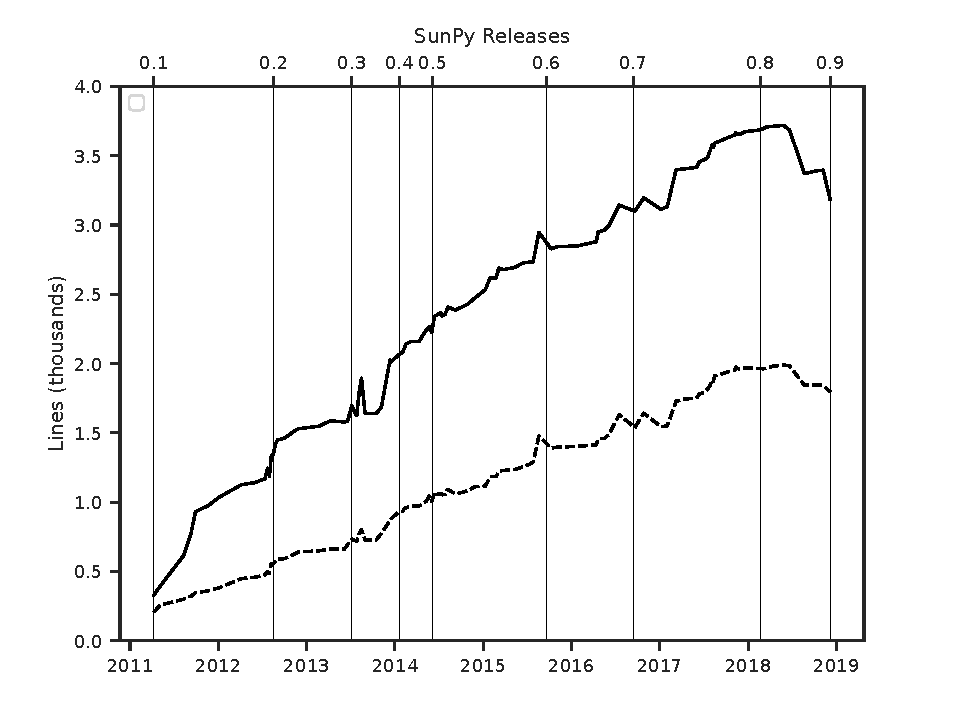
\includegraphics[width=45mm]{figures/sunpy_history.pdf} &
  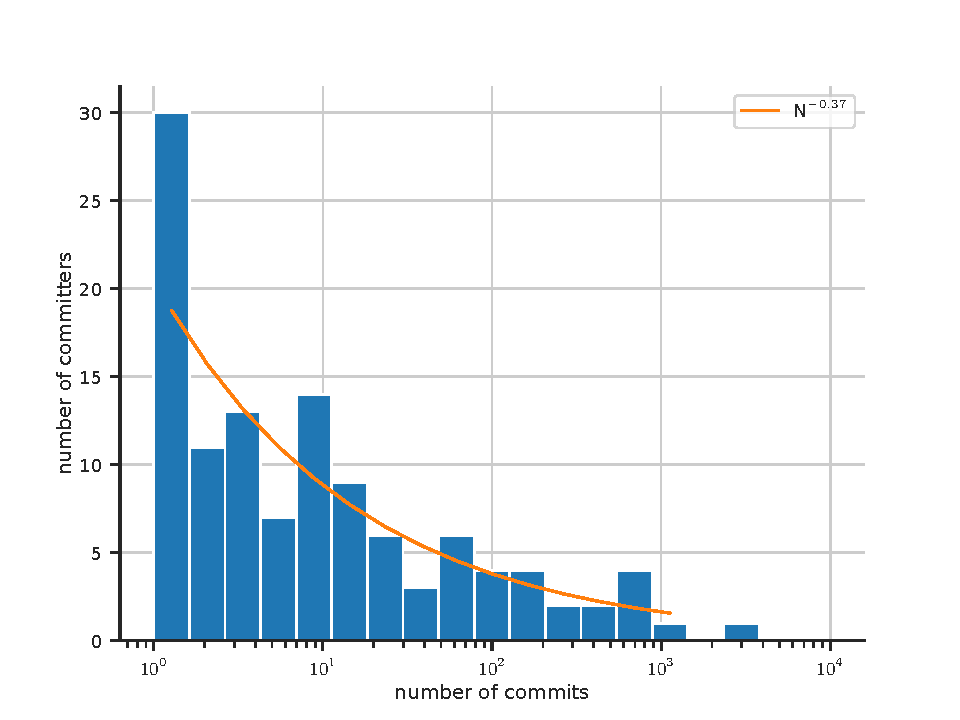
\includegraphics[width=45mm]{figures/busfactor_plot.pdf} &   
  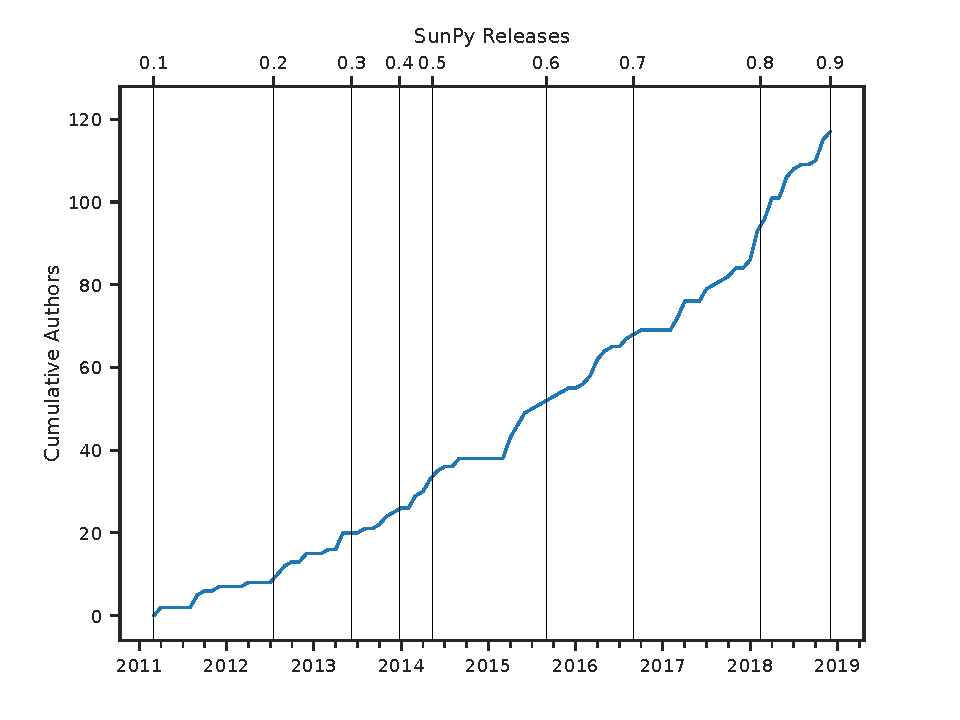
\includegraphics[width=45mm]{figures/cumulative_authors.pdf} \\
(a) & (b) & (c) \\
\end{tabular}
\caption{(a) The }
\label{fig:image2}
\end{figure}


\section{Data Types - laura}
\todo{ready for review}
\label{sec:data_types}
\todo{How many of the operating Heliophysics observatory data products do we support? https://www.nasa.gov/content/goddard/heliophysics-system-observatory-hso}
The \sunpypkg package provides core data types that are designed to provide a standardized interface to data structures across data types (images, lightcurves, spectra) as well as data sources. 
These core data types currently provided by \sunpypkg are \Map and \Timeseries classes which support 2D image data and 1D temporal data, respectively. 
They offer a consistent interface to the user allowing a simpler work-flow in the analysis and manipulation of observations. 
These objects provide visualization and basic manipulation routines with a consistent API. 
For example, metadata is provided by the \code{.meta} property, the data is stored in \code{.data}. 
They also handle all of the manipulation necessary to read data in from mission-specific files. 
The sections provide an overview of the \Timeseries and \Map objects. 

\subsection{\Timeseries - data with one temporal dimension}
\label{sec:timeseries}
\todo{ready for review}
\todo{reviewed by Steven - 22-mar-2019}
Time-series data is a fundamental observational data type. 
The \Timeseries class is designed to handle time-series data through a robust and consistent interface. 
The inherent structure of a \Timeseries object consists of times and measurements while the underlying structure used to store the data is a \code{pandas.DataFrame}. 
It supports time-series data from a wide range of solar instruments. 

The \GenericTimeSeries class is the base class of \Timeseries, which is created through the \Timeseries factory. 
A number of instruments are supported through subclassing which have instrument-specific methods for reading source files. 
Custom \Timeseries can also be made from input data in the form of a \code{pandas.DataFrame}, an \code{astropy.table.Table} or a \package{numpy} array. 

\Timeseries currently supports data sources from the following instruments: the Geostationary Operational Environmental Satellite (\textit{GOES}) X-ray Sensor (XRS), \textit{SDO} EUV Variability Experiment (EVE) \citep{woods2010extreme}, \textit{PROBA2} Large Yield Radiometer (LYRA) \citep{dominique2013lyra}, \textit{Fermi} Gamma-ray Burst (GBM) monitor \citep{meegan2009fermi}, the Nobeyama
Radioheliograph (\textit{NoRH}) \citep{nakajima1994nobeyama}, and \textit{RHESSI} \citep{lin2003reuven}. 
The \Timeseries\ object also supports the National Oceanic and Atmospheric (NOAA) Space Weather Prediction Center (SWPC) solar cycle monthly indices and predicted progression. 
These data sources are supported through a \Timeseries\ source file for each listed above. 
With this structure additional instruments and data sources can easily be added. 
\Timeseries holds meta data, stored in the \Timeseriesmetadata object. 
This functionality is designed to allow the user to create a single \Timeseries by combining multiple \Timeseries together into one, preserving the metadata relevant to each cell, column or row, concatenated into an organized fashion. 

\Timeseries also supports manipulation functionality for working with time-series data including adding new columns of data to a \Timeseries, truncating a \Timeseries over a specified time range, resampling, and creating other data products from an existing \Timeseries, such as into a \code{pandas.Dataframe} or an \code{astropy.table}. 
The \Timeseries object, similar to \Map (Section \ref{sec:map}), has it's own visualization plotting methods allowing for easy inspection of the data.

\subsection{Map - data with two spatial dimensions}
\label{sec:map}
\todo{ready for review}
The \Map class provides the functionality to store 2D data associated with a coordinate system and relevant metadata. 
A \Map object is created using the \Map factory which will produce a \GenericMap object or a subclass of \GenericMap which deals with instrument specific data.  
The main use of \Map is to store and manipulate images of the Sun and heliosphere.

A number of instruments are explicitly supported in \sunpypkg, defined within the subclass source files for each instrument source. 
The source file provides a compatibility layer which converts the specific meta data and other source-specific parameters to the standard \GenericMap\ interface. 
This also includes properties such as source-specific color tables and appropriate image scaling provided by the instrument teams. 
\sunpypkg currently supports the following instruments as part of the \GenericMap;
\begin{inparaitem}
\item \textit{SDO} - Atmospheric Imaging Assembly (AIA) \citep{lemen2011atmospheric} and the Helioseismic and Magnetic Imager (HMI) \citep{scherrer2012helioseismic}. 
\item \textit{SOHO} - Large Angle Spectroscopic COronagraph (LASCO) \citep{brueckner1995large}, Extreme ultraviolet Imaging Telescope (EIT) \citep{delaboudiniere1995eit}, and Michelson Doppler Imager (MDI) \citep{scherrer1995solar}
\item \textit{STEREO} - Extreme Ultraviolet Imager (EUVI), COronagraph 1 and 2 (COR1/2) for both \textit{STEREO} A and B \citep{howard2008sun}
\item \textit{Hinode} - X-Ray Telescope (XRT) \citep{golub2008x}
\item \textit{IRIS} Slit Jaw Imager (SJI) \citep{DePontieu2014}
\item \textit{COronal Solar Magnetism Observatory (COSMO)} -  K-coronagraph (K-Cor) all polarized brightness
\item \textit{PROBA2} - Sun Watcher using Active Pixel System detector and Image Processing (SWAP) \citep{seaton2013swap}
\item \textit{RHESSI} \citep{lin2002reuven}
\item \textit{TRACE}
\item \textit{Yohkoh} Soft X-ray Telescope (SXT) \citep{tsuneta1991soft}.
\end{inparaitem}
Helioviewer JPEG2000 image files of the above data sources are also supported by the \Map\ class.

A \sunpy \Map\ can be created either from data files from which the \Map\ factory will automatically detect the type of file, associated instrument and search the appropriate FITS keywords to infer the coordinate system. A custom \GenericMap can also be created by providing the \Map\ object with data and basic meta information.
Two additional objects based on \Map\ are also provided in \sunpy. 
The \code{MapSequence} object stores a time-ordered sequence of \Map objects.  
The data in each \Map need not have the same size (number of pixels in each direction) or view the same area of sky (field-of-view). \code{MapSequence} is useful for examining timeseries of solar images.  
The \code{CompositeMap} object permits the simple overlay and plot multiple \Map objects; such functionality is useful in displaying data from instruments with overlapping fields of view.



\section{Solar Coordinates - Will}
\label{sec:coords}
% edited by Steven C. 25-Apr-2019
% edited by Will B. 19-Apr-2019

The \package{sunpy.coordinates} subpackage provides definitions of and transformations between several reference frames commonly used in solar physics.
These reference frames and their associated transformations are implemented using the \package{astropy.coordinates} subpackage and extend \astropy's coordinate frame transformation graph to include solar coordinates.
\autoref{fig:transform_graph} shows the transformation graph between the various coordinate frames provided by \sunpy and their connection to astronomical coordinate frames.
Four solar physics coordinate frames are currently implemented: \hpc, \hcc, \hgs, and \hgc.
Each of these frames and the associated transformations are defined in \citet{2006A&A...449..791T}.
Both the \hpc and \hcc frames are observer-dependent and require the location of an observer to be specified when constructing the frame.
In the \hpc frame, the observer is at the origin of the coordinate system while in the \hcc frame the $z$-axis is defined to be parallel to the Sun-observer line.
% elaborate a bit more here as well; why are these frames useful? (split into two paragraphs)

% Description of the HCRS <-> HGS transform? - Stuart Mumford, Albert Shih? 

\begin{figure}
    % Why are the arrows between the solar frames brown and green? all black?
    \centering
    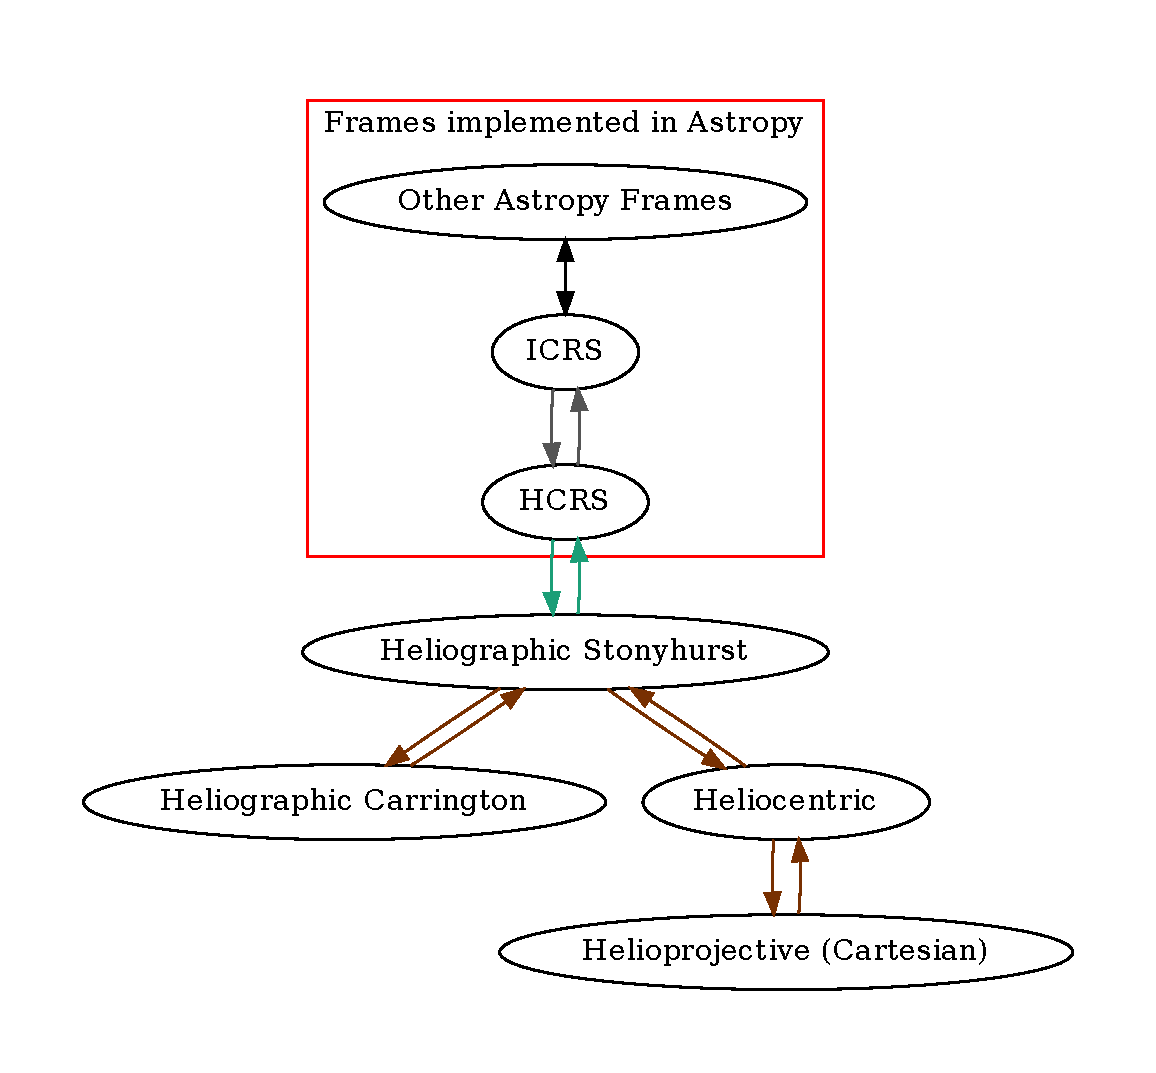
\includegraphics[width=0.75\textwidth]{figures/sunpy_frames.pdf}
    \caption{Graph of possible transformations between reference frames as implemented in \package{sunpy.coordinates}. 
    The arrows indicate transformations between the different frames. 
    Note that coordinates can be transformed to more general astronomical coordinate frames via the \hgs frame.}
    \label{fig:transform_graph}
\end{figure}

Coordinates and their associated frames are specified using an \astropy \code{SkyCoord} object \citep[see Section 3.3 of][]{astropy2018}. 
Observer location is encoded in the same way.
For example, in the \hpc and \hcc frames, the \code{.observer\_coordinate} attribute is a \code{SkyCoord} defined in the \hgs frame.
The default observer location is set to the position of the Earth as long as the time of the observation is specified.
If the time is not set the coordinate cannot be transformed to another frame unless an explicit observer is specified, as the time is required to calculate the location of the Earth.
% elaborate on this a bit

The \package{sunpy.coordinates} subpackage is most useful when combined with the \sunpycode{Map} object (see \autoref{sec:map}).
Coordinates are automatically populated when opening a FITS image using the appropriate header metadata.
This combination enables a number of number of tasks which were once cumbersome. 
A few examples are shown in \autoref{fig:coordinates_examples}.
% brief description of figures

%Just as an \code{astropy.units.Quantity} object is used to attach units to a numerical value (see \autoref{sec:units}), an \code{astropy.coordinates.SkyCoord} object includes the spatial coordinate as well as the system in which that coordinate is defined. In addition to the numerical values of the coordinate, a \code{SkyCoord} includes a reference frame or system and a representation. A reference frame describes the manner in which a point is oriented in space while a representation is a way to describe a point in a particular reference frame (e.g. Cartesian, spherical). 

\begin{figure}
    \gridline{\fig{figures/fieldlines_aia.pdf}{0.3\textwidth}{(a)}
              \fig{figures/venus_transit.pdf}{0.3\textwidth}{(b)}
              \fig{figures/cumulative_authors.pdf}{0.3\textwidth}{(c)}
              }
    \caption{(a) Several example use cases of the coordinates machinery in \sunpy. 
    (a) Field lines traced from a field extrapolation of active region NOAA XXXX computed using \package{pfsspy} overlaid on an 171 \AA image from AIA.}
    \label{fig:coordinates_examples}
\end{figure}


%Figures for this section
    % 1. transformation graph % Done
    % 2. LASCO star field (steven)
    % 3. field lines on the Sun (Will) % Done
    % 4. Venus transit image (steven)


\subsection{Solar differential coordination - Jack}
One paragraph long. 
Not clear if it needs to be in this location. 
Should it be in a map utility section?

Don't forget to refer to the figure!
An important application of....
Figure \ref{fig:diff_rot}


\begin{figure}
    \center
    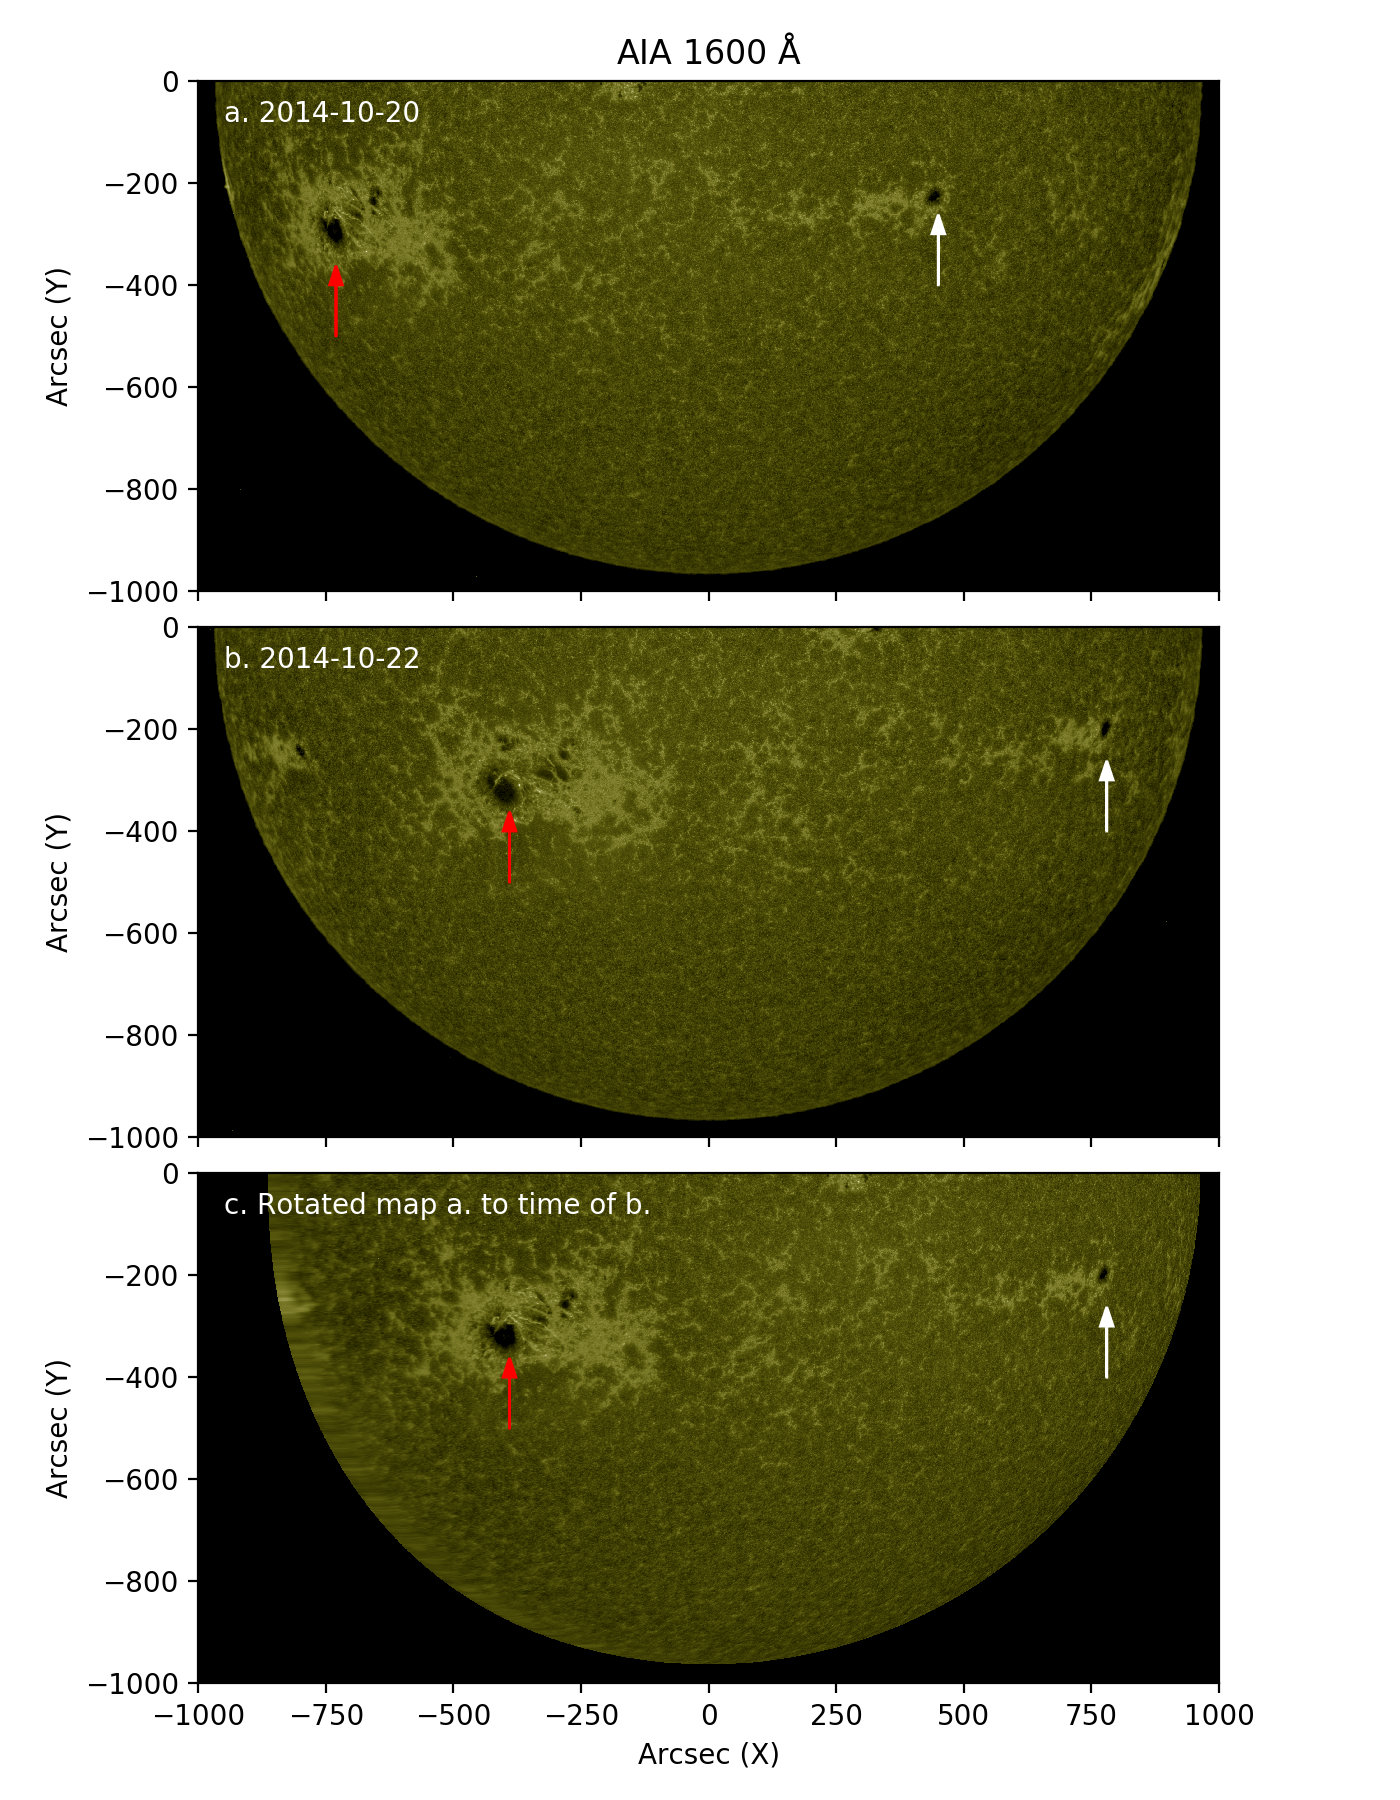
\includegraphics[width = 0.8\textwidth]{figures/diff_rot_aia1600.png}
    \caption{Example of the functionality of \sunpy to apply solar differential rotation to a Map. 
    Panels (a) and (b) show the Sun as observed in AIA 1600~\AA\ on two different days, 2014-02-20 and 2014-02-22. 
    A large sunspot group is highlighted by the red arrow, and a smaller sunspot by the white arrow. 
    Panel (c) shows the map of (a) that has been rotated differentially using \sunpy to the time of map (b).}
    \label{fig:diff_rot}
\end{figure}
\section{Data search and retrieval}
\label{sec:fido}
% edited by Steven C. 24-Apr-2019
% edited by Jack 24-Apr-2019
One of the most important tasks that must occur before any analysis can take place is to search for and retrieve data.
A particular science goal may require data from multiple data providers, each of which may have different methods of search and retrieval.  
This heterogeneity
%even in the relatively small field of solar physics
increases the effort required by scientists to get the data they need. 
In order to address this issue \sunpypkg provides a single and powerful data search and retrieval interface which can interface with all data providers. 
Referred to as \Fido, it provides a unified data search and download interface for user that simplifies and homogenizes search and retrieval to multiple data providers. 
\Fido currently supports the Virtual Solar Observatory (VSO), the Joint Science Operations Center (JSOC) (see Section \ref{sec:drms}) and a number of individual data providers that make their data available via web-accessible resources such as HTTP websites (RHESSI, SDO-EVE, NOAA GOES soft X-ray flux, PROBA2-LYRA and NOAA sunspot number prediction) and FTP sites (NOAA sunspot number, Nobeyama Radioheliograph).

A \Fido search can include multiple instruments, and can query all available data providers with a single query.  
Search queries make use of search tokens (e.g. instrument, time range, wavelength) which can be joined using Boolean operators enabling complex search queries to be constructed easily. 
The result of a query can be inspected and edited before retrieval. 
\Fido makes use of asynchronous download streams significantly improving download speeds. 

%Data downloads via the \code{Fido.fetch} method can be split up into multiple parallel streams, improving download speeds.  \Fido also handles failed data downloads: the output from \code{Fido.fetch} flags failed downloads, and passing that output back in to \code{Fido.fetch}\ allows \Fido to attempt to download those files again.

Another important aspect of data search are event catalogs. 
The primary solar event catalog is the Heliophysics Event Knowledgebase (HEK) which provides a searchable database of manually and automatically detected solar features and events such as sunspots, solar flares, coronal mass ejections, etc.  \sunpypkg provides a HEK search client which is highly flexible, allowing multiple event types and their properties to be queried simultaneously. 
For example, it is possible to search for SPoCA (\cite{2014AA...561A..29V}) active regions above a user-specified size within a given time-range.  

% sdc 24-apr-2019 - suggest that we do not mention the following as it does not add much
% to this section and should really part of the Fido anyway!
% This is a section on data retrieval, and people are using
% the helioviewer client to retrieve JPEG2000 image data.  So
% I included it, but I admit it is not a core part of SunPy's data download capability.
% Eventually SunPy's Helioviewer client should be an affiliated package and out of SunPy proper.
%The Helioviewer client permits the user to query the Helioviewer JPEG2000 image archive, download image data, and to easily construct images of solar data available at the Helioviewer archive from multiple sources.

\section{Physical Units - Bobra}
\label{sec:units}
% edited by Steven C. 23-Apr-2019

%Discuss the units SEP. discuss that we are using astropy units and provide a short description of it's capabilities. mention that sunpy.sun provides quantities with units. mention the NASA units disaster and reference units policy for NASA as reference here is a interesting reference \url{https://sma.nasa.gov/news/safety-messages/safety-message-item/lost-in-translation}

Calculations of physical quantities have traditionally been performed in software using raw numbers in the interest of speed as well as simplicity. 
Physical units have frequently been recorded in comments or in documentation which can easily lead to errors or even disaster. 
The Mars Climate Orbiter mishap in 1988 was caused by a unit discrepancy. 
The spacecraft trajectory was reported in English units instead of metric which led to the the Mars Climate Orbiter entering the Martian atmosphere well-below its intended altitude causing complete mission failure \citep{mco_mishap_report}. 
A more modern approach which ensures that physical quantities are fully described in 
software is described by \citep{Damevski2009}. 
The \sunpypkg implements this concept in all of its code through functionality provided by \astropy. 
The \code{astropy.units} subpackage implements support for physical quantities by extending \numpy array objects and define a \code{Quantity} object which consists of a number with associated units. 
Tests have shown that the overhead to using this functionality are minimal in most cases. 
It is formally mandated that all user-facing functionality provided by \sunpypkg make use of \code{Quantity} objects if appropriate. 
\code{astropy.units} also provides a tool to restrict the input in function definition to units of a particular type (e.g. length, mass). 
This is used through all \sunpypkg modules.

The \package{sunpy.sun} module contains constants, parameters and models of the Sun provided which are all provided as physical quantities as \code{astropy.units.Constants} which are \code{Quantity} with additional reference metadata. 
These include variable quantities, such as the Carrington rotation number, as well as constants, such as the solar mass. 

\todo{do we want to discuss astropy time in this section as well?}


\section{Affiliated Packages - Steven}
\label{sec:affil_package}
% edited by Steven C. 23-Apr-2019

In order to foster collaboration and code re-use, the \sunpyproj supports the concept of affiliated packages. 
These are \python package that build upon the functionality of the \sunpypkg package or provides general functionality useful to solar physics. 
Affiliated packages can also be used to develop and mature subpackage functionality outside of the constraints of \sunpypkg. 
The following requirements must be satisfied by any potential affiliated packages.
\begin{itemize}
    \item the package must make use of all appropriate features in \sunpypkg.
    \item Documentation must be provided that explains the function and use of the package, and it should be of comparable quality to \sunpypkg.
    \item A test suite must be provided to verify the correct operation of the package.
\end{itemize}
Developers can formally apply to become an affiliated package to the lead developer. 
Final approval is required by the \sunpy board for acceptance. 
Packages are re-reviewed on a yearly basis to ensure that they continue to meet the standards. 
All affiliated packages are listed on \url{sunpy.org}, are provided support by the \sunpy developer community, and advertised at conferences and workshops. 
In addition, the project further defines sponsored affiliated package which is an affiliated package whose maintenance and development is the responsibility of the \sunpy project.  

Add a line about providing a package template for affiliated packages.

The following sections provides short descriptions of the existing affiliated packages.
\label{sec:affil_packages}

\subsection{drms - Kolja Glogowski - MONICA}
\label{sec:drms}
\todo{reviewed by Steve Christe - 26-mar-2019}

The \package{drms} affiliated package provides functionality which allows for direct access to data hosted by the Joint Science Operations Center (JSOC). 
This is the primary data center for the Solar Dynamics Observatory’s (SDO)\todo{check if these instruments have already been reference before this section, and make sure that reference are provided} Helioseismic and Magnetic Imager (HMI) and Atmospheric Imaging Assembly (AIA) instruments as well as data from the Solar and Heliospheric Observatory's (SoHO) Michelson Doppler Imager (MDI) instrument. 
DRMS stands for Data Record Management System, a pSQL database that contains metadata, as well as pointers to image data, for every image taken by AIA, HMI, and MDI. 
The \package{drms} package provides access to the unique search capabilities of the JSOC which include: metadata search queries, export tailored FITS files and serve these files in a variety of methods, as well as export data as movies and images in various formats.

\todo{schriste - clean up, add more detail on that last sentence, also say what is the JSOC API interface}.

\subsection{ndcube - Dan Ryan}
\label{sec:ndcube}
% edited by Steven C. 25-Apr-2019

The \package{ndcube} package provides functionality for manipulating N-dimensional coordinate-aware data.  
It can support any combination of axis-types for example
images (2 spatial axis), images over time (2 spatial and 1 time axis), spectrograms
(wavelength and time), as well as more complex data sets such as from slit spectragraphs (wavelength, time, and spatial). 
It provides the class \sunpycode{NDCube} which is a
subclass of \astropy's \sunpycode{NDData} data container class which hold together
the data array uncertainties, and (potentially) a data mask. 
\sunpycode{NDCube} adds
support for handling world coordinate transformations through the World Coordinate System (WCS) architecture commonly used in solar physics (\todo{insert WCS reference here}). 
This package provides powerful and intuitive slicing that allow users to slice the entire dataset with a single command using either array indices or real world coordinates. 
This slices all components including the data array, and coordinates simultaneously. 
This enables users to manipulate their dataset more quickly and accurately, allowing them to more efficiently and reliably achieve their science goals and is meant to be used as a basis for more advanced and instrument specific functionality (see Section~\ref{sec:irispy}). 
Support for generalized WCS module (\todo{insert reference here}) is planned to be added in the next major release.

\subsection{radiospectra - David}


\subsection{IRISPy - Dan Ryan}
\label{sec:irispy}
% edited by Steven C. 25-Apr-2019

\package{IRISPy} provides tools to read, manipulate and visualize data from the Interface Region Imaging Spectrograph (IRIS; \citealt{DePontieu2014}). 
IRIS is a NASA Small Explorer mission which has two instruments; a slit-jaw imager (SJI) and a rastering slit spectrograph (SG). 
The \package{IRISPy} is limited to reading level 2 data for either of these instruments. 
This package provide data classes \sunpycode{IRISMapCube} and {IRISSpectrogramCubeSequence} which hold data from SJI and SG respectively.
Built on top of the functionality provided by \package{ndcube} (see Section\~ref{sec:ndcube}) they link the main observations, metadata, uncertainties, data unit, mask, and WCS transformations and provide easy slicing of the data in any axis. 
Measurement uncertainties accounting for Poisson statistics and readout noise are automatically calculated while a mask identifies what pixels of the data array are exposed to the Sun. 
The mask facilitates basic operations, e.g.\ mean, max, etc., and removes bad pixels from the color table in visualizations.


%This is useful when one axis represents two coordinates, one of which is parallel while the other is not.
%For example, a scanning slit-spectrograph can scan its slit through a number of positions along the x-axis, before moving back to the original position and repeating the process.
%Therefore the sequence axis is parallel, as the scans are sequential in time, but also perpendicular because in that the scan number represented by the sequence axis is not related to the spatial position of the slit represented by the x-axis of the constituent \sunpycode{NDCubes}. 
%Users may want to think of the x-axis as time, in which case the \sunpycode{NDCubeSequence} is like an ND dataset, then instantly change to thinking about the x-axis as slit position, in which case the \sunpycode{NDCubeSequence} is better represented as an N+1D dataset.
%To achieve this model in the past, the data would have to be duplicated and placed into two separate objects with different shapes and sets of coordinate transformations.
%This paradigm requires both objects be kept consistent, leading to a greater workload and potentially more errors.
%By contrast, \sunpycode{NDCubeSequence} makes this possible for a single object, speeding up analysis, minimizing memory resources, and reducing the potential for errors.

%Moreover, because the data unit is linked to the object, it is always obvious what unit the data is in. This saves scientists the hassle of performing important, but laborious and repetitive data conversions and avoid confusion by always tracking the unit of the data through those conversions. This leads to more efficient and accurate science.
\section{Community - Bobra}
\label{sec:community}

%guidelines:
%start with code of conduct. 
%discuss the need for community to support projects. %summarize tutorials given at conferences. 
%go over communication tools provided. 
%talk about the board and how it provides a place for community members to contribute leading the project. discuss code of conduct. 
%mention how many people have contributed and how %contributions are rewarded. 
%mention numfocus award. 
%google summer of code and ESA summer of code.

\subsection{Participation}
The SunPy community follows an open development process, wherein everyone is welcome to contribute code, raise issues, and provide feedback. 
As detailed in SunPy Code of Conduct, the community encourages everyone, including newcomers, to join this process, and strives to create an create an open, considerate, and respectful environment for all. 
As part of the open development process, the SunPy community maintains many active daily communication channels. 
Users can connect with the community through mailing lists, on an open-source protocol for real-time chat called matrix.org, or by attending weekly telecons.
The SunPy community also fosters code development for newcomers and experienced programmers alike through tutorials, summer programs, and mentorship. 
SunPy community members voluntarily organize tutorials at various conferences and workshops, including AAS Solar Physics Division meetings. 
The SunPy Project also participates in two summer of code programs, which offer students stipends to write code for open-source projects, via the OpenAstronomy umbrella organization. 
Since 2013, 16 students contributed to SunPy through the Google Summer of Code (GSoC) program. 
Since 2011, 7 students contributed to SunPy through a similar program funded by the European Space Agency called The ESA Summer of Code in Space. 
Many SunPy community members served as mentors for these students. 

In 2018, NumFOCUS, a 501(c)(3) public charity which collects and manages tax-deductible contributions for many open-source scientific software packages such as NumPy and AstroPy, gave GSoC student Vishnunarayan K. I. an award for exceptional contributions to the open source scientific software ecosystem for his efforts to update SunPy with a modern astronomical time system.

As of the publication of this paper, the SunPy community consists of 35 active developers, 111 contributors, and an average of approximately 200 commits to the code base on a monthly basis. 
The commit history for the entire project is openly available, as are statistics for the number and frequency of commits per developer. 
Each developer and contributor to the \sunpy project is recognized for their work by name on papers, posters, and release notes.
\section{Infrastructure - Stuart}
\label{sec:infrastructure}
% edited by Steven C. 23-Apr-2019

\subsection{Releases and Versioning - Nabil}
% my formatting sucks here, sorry Steve.

SunPy has been releasing on a ill-defined schedule but for 1.0 and on-wards, it was decided to follow a release schedule. 
There will be two planned releases of \sunpypkg per year with 6 months between these releases around the months of May and November.
This is to align the release with release cycles of upstream packages such as Astropy.

Furthermore, each release of \sunpypkg will fit into one of two categories: a Long Term Support (LTS) release and a short-support or non-LTS release.
The main difference is the differing amounts of time that a release will be supported by bug fixes and documentation upgrades. 
The first release of the year shall be a non-LTS release, which shall be supported for 6 months or until the next release.
The second release of the year will be an LTS release and will be supported for 12 months or until the next LTS release.

\sunpypkg will follow the following versioning system: ``X.Y.z", where the three components have the following meaning.
``X" is the LTS version number, this will be incremented with every LTS.
``Y" is the release counter, this will be 0 for LTS releases and increment for each intermediate release.
``z" is the bug fix number, and is to be incremented for any bug-fix releases.

An example release sequence, following this scheme, would look like this:

\begin{itemize}
\itemsep0em
\item 1.0.0 is an LTS release, released November 2019.
\item 1.1.0 is a short support release, released May 2020.
\item 1.0.1 and 1.1.1 are bug-fix releases, released June 2020, to fix a current bug and back-port the fix to the LTS version.
\item 2.0.0 is an LTS release, released November 2020.
\end{itemize}

One benefit of users using an LTS release is that it will provide warnings for any functionality that will be changed or removed for the next LTS release.
Where as changes to the code that could break existing scripts, will not happen until the next LTS release but could happen on the non-LTS releases.
This provides a stable base for long term \sunpy users.

\subsection{Continuous Integration - Nabil}
The \sunpyproj follows common practices and makes extensive use of continuous integration
which refers to the practice of automated testing and code change inspection.  
Any and all proposed code contributions to \sunpypkg trigger test suits to be run on a number of free services which integrate into the \github website. 
These services provide the first review of all new code and therefore maintain the integrity of the package which makes it easier for new contributors to understand the impact of their changes.

\sunpypkg's test suite can be broken down into three broad categories: offline, online and figure tests. 
Offline test suite checks the majority of the codebase. 
Online tests specifically checks code that contacts generalized data service providers such as the VSO \todo{(predefined else where?)} or JSOC as well as specific data providers like GOES or NOAA. 
These tests depend on the availability of these online services. 
Finally figure tests check code that generate plots and will generate a failure if the image has changed. 
This enables high level functionality checks.

\sunpy makes use of the following online services:

\begin{itemize}
\item \href{https://azure.microsoft.com/en-gb/services/devops/pipelines/}{Microsoft's Azure pipelines}: Runs the entire test suite on each operating system (Windows, Mac, Linux).
\item \href{https://circleci.com}{circleci}: Runs the library's documentation, a special 32bit build and the figure tests.
\item \href{https://travis-ci.org}{Travis CI}: Runs the entire test suite on a daily cadence.
\item \href{https://codecov.io/}{Codecov}: Provides code coverage metrics.
\end{itemize}

% sdc 24-Apr-2019 the following is not a test suite
%\item \href{https://readthedocs.org/}{Read the Docs}: This is where our \href{http://docs.sunpy.org/en/stable/}{online documentation} is hosted, they also build the documentation in the process.
% Nabil 04-May-2019 sure but I think its important to add it somewhere. 
% We do use it a lot and it should be listed somewhere.
\section{Conclusion - Steven}
\label{sec:conclusion}
% edited by Steven C. 25-Apr-2019
% sdc still needs significant work...

Development of the \sunpypkg core package has been going on now for 8 years with the project adopting a formal organization to lead the project 5 years ago. 
In that time, the core package has grown to provide significant functionality for a growing number of users. 
Significant additional features are currently missing and either under active development on are planned for development. 
These include support for spectra and spectral fitting, support for multi-dimensional datasets (e.g. slit spectrographs, radio spectrograms), providing a standardized approach to metadata.
The board structure is meant to ensure that the leadership of the project remains within the community and reflects a broad spectrum of the community.
The project has adopted an official Code of Conduct\footnote{\url{http://docs.sunpy.org/en/stable/coc.html}} whose purpose is to ensure that the \sunpy community is positive, inclusive, successful, and growing. 
The three primary aspects that are encouraged in each community member is to be open, considerate and respectful. 
A significant obstacle to the growth of the developer community has been the difficulty in providing the appropriate tools and guidance to users to contribute to \sunpypkg. 
The conversion from user to contributor requires significant additional skills which are not prevalent in the solar community including knowledge of version control, writing user documentation and unit testing. 
This is in addition to the not insignificant effort of refactoring code for public use. 
Finally, informal surveying suggests that the scope of the \sunpypkg package is not clear which likely disincentive contributions. 
The \sunpyproj is now a member of the Python in Heliophysics Community (PyHC)\footnote{\url{heliopython.org}}, whose members contribute to a collection of over fifty Python packages that span every sub-discipline within heliophysics which includes solar physics. 

\section{acknowledgements}
We would like to acknowledge financial contributions by Google as part of the Google Summer of Code program.

\acknowledgments
\software{Astropy \citep{astropy2018}}

\bibliography{bibliography}

\end{document}
